\documentclass[12pt, oneside]{article}   
\usepackage{textcomp}

\usepackage{listings}
\lstset{language=R,literate={<-}{{$\gets$}}1}

\usepackage[a4paper,bindingoffset=0.2in,%
            left=0.75 in,right= 0.75 in,top= 0.75 in,bottom=0.75in,%
            footskip=.55in]{geometry}

                		
\geometry{letterpaper}                   		
\usepackage{amsmath}
\usepackage{graphicx}

\setlength{\parindent}{0pt}

\title{Bayesian Analysis of Randomized Controlled Trials}
\author{Julian Bautista, Alex Pavlakis, Advait Rajagopal}
%\date{\today}		
			
\begin{document}
\maketitle

\abstract{}	

\newpage 

\tableofcontents
\newpage

\section{Introduction}
Set up the paper. This is me learning GitHub.

\section{Bayesian Data Analysis}
BDA and inference is the process of developing and fitting a probability model to data. The result is a probability distribution of model parameters from which one can evaluate the fit of the model to  data and make predictions for new observations [Gelman et. al 2013; Gelman and Hill 2007].\\
\\
Below we list the three steps to BDA.  Each is explained in detail in section 2.1, 2.2 and 2.3 respectively.
\begin{enumerate}
\item{\textbf{Build a model:} Set up a probability of model of parameters of interest conditional on observed data and all available information about the problem.}
\item{\textbf{Fit the model:} Calculate the distribution of the model parameters, given the observed data. This is called the \textit{posterior distribution} of the parameters.}
\item{\textbf{Evaluate the model}: Check the fit of the model, whether the conclusions are sensible and how sensitive they are to modeling assumptions. Expand or alter the model and repeat the steps if needed .}
\end{enumerate}

\subsection{Model development}
Model development involves setting up a joint probability distribution that accounts for all observed data and unobserved parameters. The model should include all knowledge of the experiment or data collection process and should be logically consistent with scientific nature of the problem at hand. We approach model development in three steps.
\begin{enumerate}
\item{\textbf{Exploratory Data Analysis}: Look at your data.  What stands out?  What \emph{distributions} do different variables appear to take on?  What seems important?  What variables are correlated?  Answers to these questions are essential to specifying a the following two model components.  For most scientific problems there is no one-size-fits all model or reliable automated model choosing program; you have to get your hands dirty.}
\item{\textbf{Setting up a Likelihood Model}: Choose a model that represents the relationship between your data and parameters of interest.  For instance, if your outcome variable is binary (0 or 1), a logistic regression framework may be appropriate.}
\item{\textbf{Choosing a prior distribution}: Specify assumptions and knowledge about parameters of interest explicitly in the form of prior distributions.  For instance, if a coefficient of interest \emph{must} be between 0 and 1, you may want to set a \emph{Beta} distribution on that coefficient.  If you believe that a coefficient is close to zero, but may be positive or negative, you may want to assign a \emph{Normal}(0, 1) prior distribution to it.}
\end{enumerate}

To make this concrete, let $\theta$ be a parameter of interest and $y$ be data from which we want to estimate $\theta$.  Then the prior distribution and likelihood are, respectively:
\begin{align}
p(\theta) \\
p(y | \theta)
\end{align}

Bayesian inference involves multiplying these distributions together according to a fundamental rule of probability to estimate a \emph{posterior distribution} of parameters conditional on data.
\begin{align}
p(\theta | y) \sim p(\theta) p(y |\theta)
\end{align}

The Bayesian approach combines data and prior information in a way that can yield more precise inferences than either on its own.


\subsection{Model estimation}
The goal of model estimation is to calculate the \textit{posterior distribution} of parameters; the conditional distribution of the parameters given the observed data. The posterior distribution is obtained by simply multiplying the prior and likelihood to get joint probabilities and then normalizing to get posterior probabilities. Calculating the posterior analytically is often difficult and leads to intractable integrals with no closed-form solution. Standard practice is to use MCMC sampling methods to approximate the posterior up to a normalizing constant and sample from it. There are some other approaches to calculating the posterior distribution, but those are beyond the scope of this paper. Using these posterior distributions we can now predict and simulate replicated data from our model, which leads us to section 2.3. 
\\

\subsection{Model checking, comparison and expansion}
We begin evaluating the performance of our model by ensuring that it converges on robust parameter estimates and that the results make sense given what we know about the observed data and the problem itself. We also need to see how sensitive our results are to the modeling assumptions and the priors. Sometimes using stronger priors can help with convergence and more stable results. We use our posterior distributions of the parameters to check our model by carrying out \textit{posterior predictive checks}. This could be graphical checks where we simulate ``fake" data from our model and compare it graphically to the raw data. We could also use certain test statistics and compare the values of those statistics across models and see how close they are to the ground truth obtained from the observed data itself. Based on the fit of the model, we can either expand the model to include more parameters, predictors or change the model and reevaluate performance. We are not looking to explicitly choose the ``right" model but are interested to learn where each of our approaches and models might be lacking and make these shortcomings explicit while trying to improve them.


\section{Comparison of Bayesian Data Analysis to Other Methods}
There are two primary benefits to a Bayesian approach for RCT. First is the improvement of predictions through the use of a greater amount of information within the models. Second is a greater level of transparency through explicit assumptions. This section will end with a discussion of some of the risks of Bayesian approaches.
\subsection{Better Prediction}
As discussed earlier, the choice of a prior distribution is a critical assumption that directly affects the results of the analysis. Bayesian analysis lends itself well to the infinitely many distributions that can be used. But beyond the choice of a distribution, the specifications of hyper-paramaters of these distributions allow for the usage of data that exists beyond that which was collected within the study. 

Data does not live only on the spreadsheet. It is contained in the researcher's knowledge of the literature, the data generating process, and anything else that is relevant. This can include common sense knowledge such as the understanding that estimates on ratios will be between 0 and 1, or it could be an expected estimate based on previous studies done. Regardless of the source of the information, knowledge about an estimator can be translated into the prior to improve accuracy. 

One of the most powerful hyperparameter specifications is to specify a hierarchical model to allow partial pooling. Hierarchical data structures include any data that can be represented in categories. In a non-Bayesian scenario, there are two choices a researcher has: a complete pooling model, and a no pooling model. With complete pooling, the data is treated essentially as exchangeable, thus ignoring the uniqueness of categories. With no pooling, each category is treated as independent of the others, thus ignoring the interrelatedness of each of the categories. Setting a hyperparameter as a distribution allows us to say that our relevant parameters have a common mean, but are each different from one another. This partial pooling is often more accurate as it takes into account both the uniqueness and interrelatedness of categories within a hierarchical model.

The Bayesian approach also allows the researcher to break free from degrees of freedom... Allows us to use interaction variables and stuff

\subsection{Better Transparency}
Bayesian Approaches are so transparent that this section is written in transparent digital ink.

\subsection{Risks to a Bayesian Approach}
There are none. Move on.
\section{Reproducibility}
Describe the philosophy and importance of reproducibility.  

Describe the steps of making research reproducible (e.g. sharing code, sharing data, explicitly specifying model, etc.)

\section{Impact of Smartphone App on Eating Behavior}

Hildebrandt et all (2017) conducted an experiment to test whether the Noom Monitor, a smartphone application, could augment the effect of in-person therapeutic treatment on binge eating behavior.  The treatment, known as \emph{guided self-help treatments based on cognitive-behavior therapy} (CBT-GSH), had been shown in previous research to reduce binge eating behavior by 10-50\%.  The Noom Monitor application was designed to facilitate CBT-GSH.  For this example, we consider two research questions from the experiment:
\begin{enumerate}
\item{Is CBT-GSH more effective at reducing binge eating behavior when facilitated by the Noom Monitor?}
\item{Does the effect of the Noom Monitor vary over time?}
\end{enumerate}

\subsection{Experimental design}

66 men and women with Bulimia Nervosa (BN) or Binge Eating Disorder (BED) were randomly assigned into two treatment conditions: CBT-GSH (N= 33) or CBT-GSH + Noom (N=33).  Therapy lasted for 12 weeks.  Assessments were conducted at weeks 0, 4, 8, 12, 24, and 36.  The primary outcome was Objective Bulimic Episodes (OBE).  

\subsection{Exploratory data analysis}

\begin{figure}
\centering
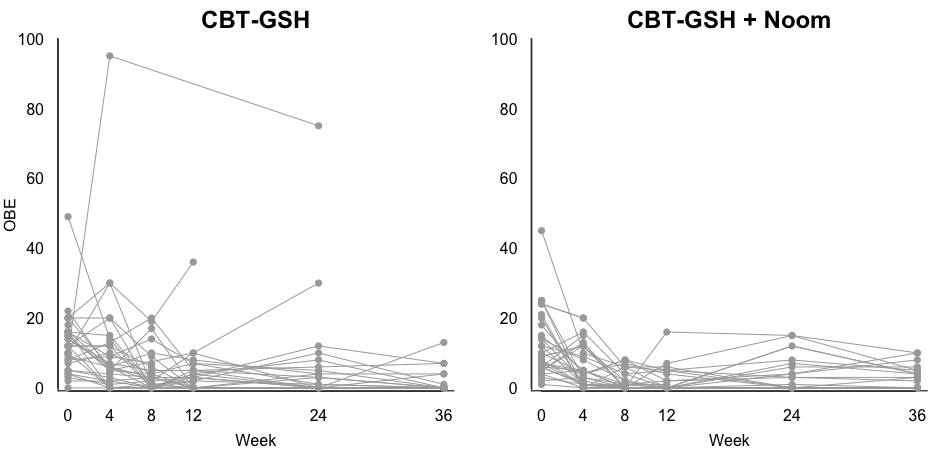
\includegraphics[width=\textwidth, height=\textheight, keepaspectratio]{Noom_paths.png}
\caption{\emph{Plots display OBEs over time for each individual in the CBT-GHS groups (left panel) and CBT-GHS + Noom group (right panel).}}
\end{figure}

Figure X displayes OBEs per week for each individual in both treatment conditions.  A few aspects of the data immediately stand out, which suggest that any model should account for individual-level effects and time-level effects, and should let treatment effects vary over time.  
\begin{itemize}
\item{The number of OBEs decreases over the course of the treatment for almost all subjects}
\item{The biggest decreases in OBEs appear to occur in the early stages of treatment}
\item{The primary sources of variation in OBE appear to be \emph{between people} and \emph{over time}.}
\end{itemize}

\newpage

\begin{figure}
\centering
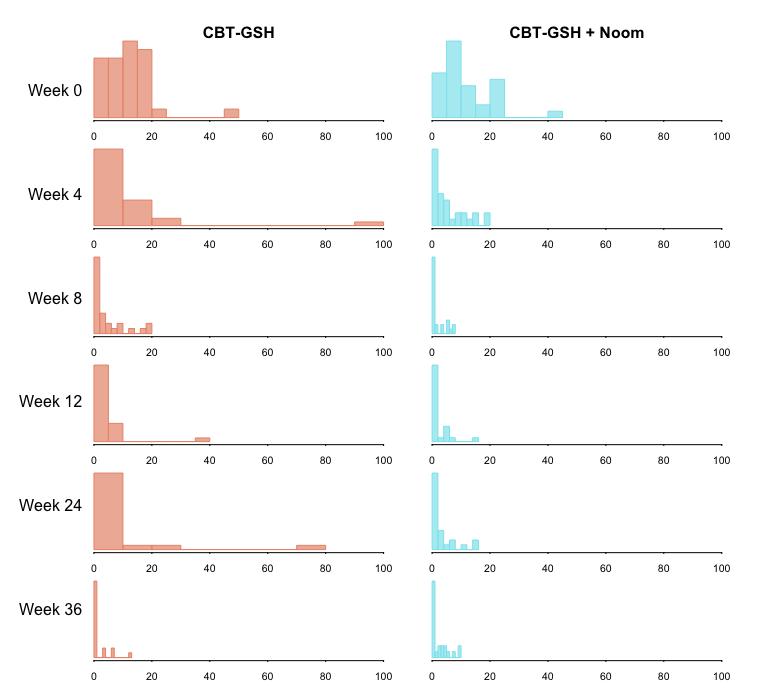
\includegraphics[width=\textwidth, height=\textheight, keepaspectratio]{noom_hist.png}
\caption{\emph{Histograms display the distribution of OBEs in each condition in each week.}}
\end{figure}

Figure Y displays the distribution of OBEs in each condition in each week.  We notice three characteristics of the data from these histograms.
\begin{enumerate}
\item{The distributions appear to condense around zero for both conditions over time} 
\item{The distributions in the CBT-GSH condition appear to have longer tails than those in the CBB-GSH+Noom condition}
\item{OBEs are count data; they must be nonnegative integers.}
\end{enumerate}
These three characteristics suggest that the appropriate model for OBEs is the Poisson distribution, because it is restricted to nonnegative integers and can concentrate its density around low numbers with a long tail.

\subsection{Model development}

\begin{table}[t]
\centering
\begin{tabular}{r l}
  Source of Prior Information &  \\ 
  \hline  \vspace{0.25em}
  Experimental Design & Outcome variable is nonnegative integers \\
  \vspace{0.25em}
  Literature & Effect size is close to zero \\
  Exploratory Data Analysis & There is variation in OBEs at the individual level \\
					  & There is variation in OBEs over time \\
                                            & Treatment effects may vary over time \\
    \hline
\end{tabular}
\caption{\emph{Sources of prior information.}}
\end{table}


We analyze RCTs by modeling the outcome of interest (in this case OBE) as a function of the treatment and all available pre-treatment covariates.  The coefficients associated with the treatment reveal the average treatment effects.  Inclusion of all available pre-treatment covariates accounts for variation in the outcome variable, decreasing uncertainly around treatment effects and providing the model with more predictive power.  We conduct \emph{intent-to-treat} analysis, meaning that our inferences will be based on initial treatment assignment, and will not account for mid-experiment dropouts.  
\\

The outcome variable is restricted to be nonnegative integers, so we fit a Poisson regression model, with hierarchies on individuals, time periods, and treatment effects.  For each individual in each time period, the number of OBEs follows a Poisson distribution, with a mean dependent on the characteristics of the individual and the time period.  

\begin{align}
OBE_{i,t} &\sim Poisson(\lambda_{i,t}) \\
\lambda_{i,t} &= exp(\alpha_i + \beta_t + \gamma_tT_i + X_i\theta) \\
T_i &=
    \begin{cases}
      0, & \text{if}\ CBT-GSH \\
      1, & \text{if}\ CBT-GSH + Noom \\
    \end{cases}
\end{align}

$\alpha$ is an individual-specific intercept, $\beta$ is a time-specific intercept, $\gamma$ is a time-specific treatment effect, $T$ is a treatment indicator, $X$ is a matrix of individual level covariates (age, sex, race, etc), and $\theta$ is a vector of effects. Subscripts $i = 1, ..., 66$ indicate individuals and subscripts $t = 0, 4, 8, 12, 24, 36$ indicate time periods.
\\

We believe that individual-level intercepts are simultaneously unique to the individual and common to the population; that is, each individual has their own baseline predilection to engage in eating disorder behavior, but their baseline predilections are not drastically different from each other.  We operationalize this concept by modeling all individual-level intercepts as coming from a common distribution, with \emph{hyperparameters} $\mu_{\alpha}$ and $\tau_{\alpha}$.
\begin{align}
\alpha_i \sim Normal(\mu_{\alpha}, \tau_{\alpha}) \ \forall \ i \in 1,...,66
\end{align} 

Similarly, we believe that time-specific treatment effects may be unique to each period but similar over time. We operationalize this concept by modeling all time-specific treatment effects $\gamma$ as coming from a common distribution, with \emph{hyperparameters} $\mu_{\gamma}$ and $\tau_{\gamma}$.
\begin{align}
\gamma_t \sim Normal(\mu_{\gamma}, \tau_{\gamma}) \ \forall \ t \in 0, 4, 8, 12, 24, 36
\end{align} 

$\mu_{\gamma}$ is the \emph{grand mean}, the overall treatment effect; $\tau_{\gamma}$ is the variation in treatment effects over time; and each individual $\gamma_t$ is a time-period specific treatment effect.  This approach has a natural smoothing effect: any extreme estimates of $\gamma_t$ will be partially-pooled back toward the grand mean $\mu_{\gamma}$.
\\

We assign the following prior and hyperprior distributions:
\begin{align}
\mu_{\alpha} &\sim Normal(5, 5) \\
\tau_{\alpha} &\sim Cauchy^+(0, 30) \\
\mu_{\gamma} &\sim Normal(0, 5) \\
\tau_{\gamma} &\sim Cauchy^+(0, 30) \\
\theta &\sim Normal(0, 1) \\
\end{align}

The normal distributions around the individual and treatment effects allow us to guide the model to the appropriate range of parameter values, but with wide enough variance (5 in each case) to let the model find its own way in that range.  Half cauchy priors on the variance parameters are weakly informative, with much of their mass around zero but gentle slopes in their tails, which have been shown to be effective prior distributions for variance parameters (Gelman, 2006).

\subsection{Model estimation}
We estimate this model with \emph{Hamilton Monte-Carlo} in Stan.  Model code is appended to this document.  We find that the model converges with four chains of 2000 iterations each (see table M).  

\subsection{Posterior predictive checking}

\begin{figure}
\centering
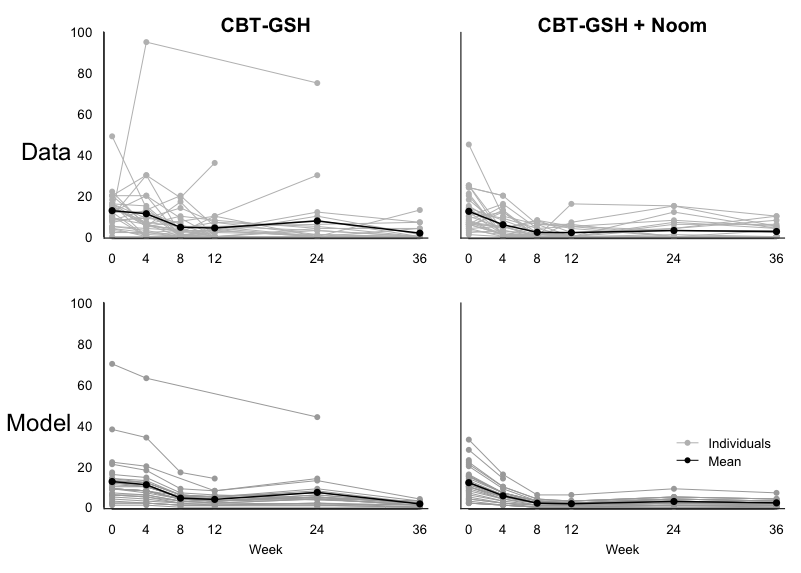
\includegraphics[width=\textwidth, height=\textheight, keepaspectratio]{ppc_sims.png}
\caption{\emph{Upper plots show OBEs in each period for each individual in both treatment group, with black lines representing means.  Lower plots show modeled OBEs for each individual in each treatment group, with black lines representing modeled means.  The model appears to be able to recover OBEs over time fairly well for both treatment conditions.}}
\end{figure}

Before using our model to make inferences about time-specific treatment effects, we check its fit by comparing model-simulated OBE to data OBE.  If model simulations do not track the data well, we may want to revisit our model's assumptions before trusting its inferences.  If the model's simulations recover patterns in the data, we are more inclined to trust its inferences.  
\\

Figure Q displays OBEs in each period for each individual in each treatment group, from raw data (upper plots) and model simulations (lowers plots).  Black lines display means for each.  This suggests that the model is broadly able to pick up on the key variables that determine OBE over time for the duration of this experiment.
\\

Another way to check the fit of the model is by comparing simulated data directly against the raw data.  Figure P shows this for both treatment conditions.  Simulated data for the Noom condition appears to better track the raw data than simulated data for the no Noom condition.  This is unsurprising, since the no Noom condition tended to have more outliers, which we would not expect (or want) our model to pick up perfectly from such a small sample.  
\\

\begin{figure}
\centering
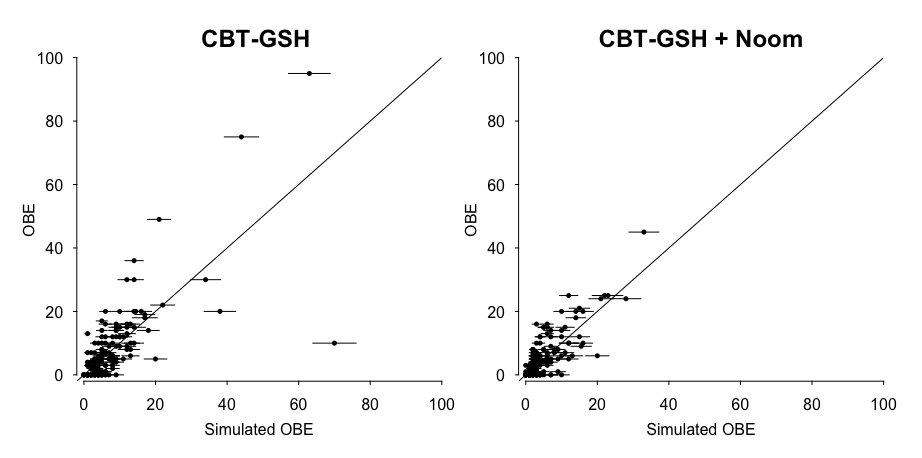
\includegraphics[width=\textwidth, height=\textheight, keepaspectratio]{obe_ppcs.png}
\caption{\emph{Plots display siulated OBEs to raw data for both treatment conditions.  Model simulations appear to match the raw data well, particularly for the Noom condition, which had fewer outliers.}}
\end{figure}

We conclude our model evaluations by mapping modeled density curves for each condition in each time period over the histograms in figure Y.  Figure BB shows that our model is able to broadly pick up on the patterns in the data over time and between treatment conditions.

\begin{figure}[h]
\centering
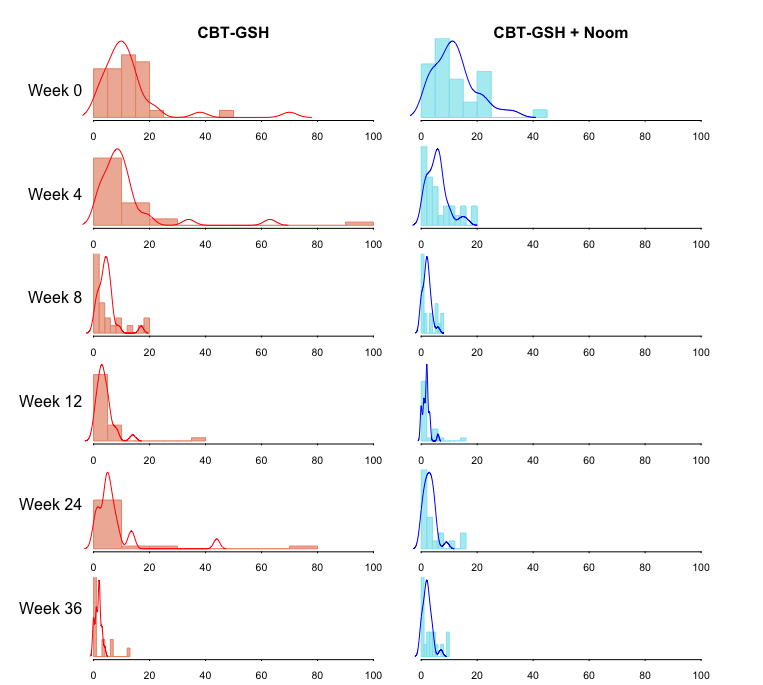
\includegraphics[width=\textwidth, height=\textheight, keepaspectratio]{ppc_hist_dens.png}
\caption{\emph{Histograms display the distribution of OBEs in each condition in each week.}}
\end{figure}

\subsection{Results}
Model results are displayed in table M.  Results suggest that using the Noom Monitor smartphone application during CBT-GSH may slightly decrease OBEs.  There some evidence that the treatment effect varies over time, with the Noom effect being slightly more pronounced during the later stages of therapy.
\\

Figure R displays modeled OBE for both treatment groups (upper plot) and smoothed treatment effects (lower plot).  In each measurement period, simulated OBE are higher for the No Noom condition than for the Noom condition, with some of the difference likely attributable to use of the Noom Monitor smartphone app.  

\begin{table}[t]
\centering
\begin{tabular}{r c c c c c}
  \hline
 & mean & 25\% & 50\% & 75\% \\ 
  \hline
  $\gamma_0$ & 0.18 & -0.45 & 0.15 & 0.78   \\ 
  $\gamma_4$ & -0.43 & -1.05 & -0.46 & 0.16   \\ 
  $\gamma_8$ & -0.70 & -1.33 & -0.71 & -0.10   \\  
  $\gamma_{12}$ & -0.65 & -1.28 & -0.68 & -0.04   \\  
  $\gamma_{24}$ & -0.72 & -1.34 & -0.75 & -0.11  \\  
  $\gamma_{36}$ & 0.21 & -0.42 & 0.19 & 0.82  \\ 
  \hline \hline
  $\mu_{\gamma}$ & -0.34 & -0.98 & -0.36 & 0.26  \\ 
  $\tau_{\gamma}$ & 0.64 & 0.43 & 0.56 & 0.77  \\ 
   \hline
\end{tabular}
\caption{\emph{Table displays model results for Noom effects in all six time periods and grand mean and variance parameters.}}
\end{table}


\begin{figure}[h]
\centering
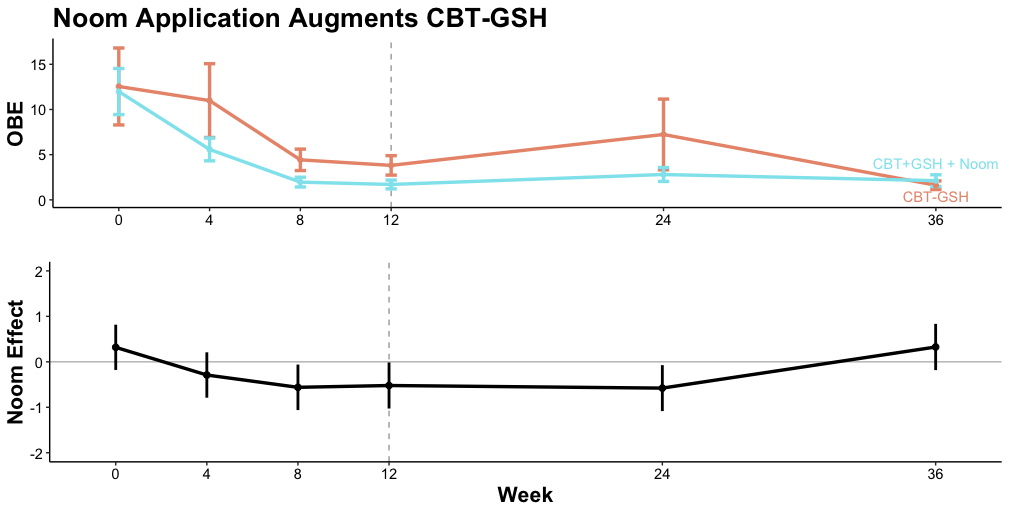
\includegraphics[width=\textwidth, height=\textheight, keepaspectratio]{noom_effect.png}
\caption{\emph{Upper plot displays modeled OBEs in each time period for the Noom (blue) and no Noom (orange) conditions with 95\% intervals.  Lower plot displays modeled treatment effects in each period,with 50\% intervals.}}
\end{figure}


\section{Conclusion}
So awesome

\section{Appendix}
All the math goes here

\end{document}